
\begin{figure}[H]
  \centering
  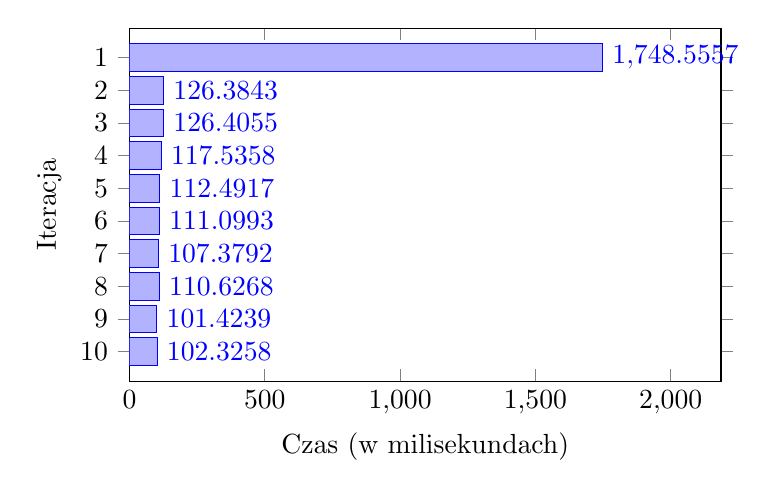
\begin{tikzpicture}
  
    \begin{axis} [
      xbar = .05cm,
      nodes near coords,
      nodes near coords style={
        /pgf/number format/precision=4,
      },
      xmin = 0,
      ytick = data,
      enlarge x limits = {value = .25, upper},
      symbolic y coords = {10,9,8,7,6,5,4,3,2,1},
      xlabel=Czas (w milisekundach),
      ylabel=Iteracja,
      width=0.75\textwidth,
      height=0.5\textwidth
    ]
    
      \addplot coordinates {(1748.5557000041008,1) (126.38430005311966,2) (126.40549999475479,3) (117.53579998016357,4) (112.49169999361038,5) (111.09930002689362,6) (107.3792000412941,7) (110.62680000066757,8) (101.4239000082016,9) (102.32580000162125,10)};
      
    \end{axis}
  
  \end{tikzpicture}
  \caption{Wynik testów przykładu 4 [\ref{lst:wydajnosc-przyklad-p-4}]}
  \label{fig:wynik-przyklad-3}
\end{figure}
